\documentclass[12pt,a4paper]{article}
\usepackage{iftex}
\ifXeTeX
  \usepackage{fontspec}
  \usepackage{xeCJK}
  \setmainfont{Times New Roman}
  \setsansfont{Arial}
  \setmonofont{Consolas}
  \setCJKmainfont{SimSun}
  \setCJKsansfont{Microsoft YaHei}
  \setCJKmonofont{FangSong}
\else
  \usepackage[UTF8]{ctex}
\fi
\usepackage{amsmath,amssymb,graphicx,bm} % amssymb provides \longmapsto
\usepackage{siunitx}
\usepackage{geometry}
\geometry{margin=2.5cm}
\usepackage[hidelinks]{hyperref}
\usepackage{mathrsfs}
\usepackage{float}

\title{柔性臂串联系统动力学建模与推导}
\author{chen lin}
\date{2025.10.8}

\begin{document}
\maketitle

\tableofcontents

\clearpage

\section{符号说明与系统概述}
\begin{itemize}
  \item 每一级柔性臂包含三根驱动杆及一个顶盘，广义位移记作 $\bm h = [h_1, h_2, h_3]^\top$，对应杆长方向的伸缩量。
  \item 令 $\dot{\bm h}$ 为一阶导，系统状态向量按照 $\bm q = [\bm h^\top,\, \dot{\bm h}^\top]^\top$ 排列。
  \item 底盘至第一顶盘的初始高度 $h_0$，底座等边三角形边长 $L_0$。
  \item 坐标系采用 $\{\mathcal{W}\}$（世界坐标）与各级局部坐标 $\{\mathcal{B}_s\}$，所有齐次变换均以 $4 \times 4$ 矩阵表示。
\end{itemize}

串联 $S$ 级柔性臂时，每一级的状态变量彼此独立，但其末端位姿需经由齐次变换累乘以得到最终顶盘位姿。下文先推导单一级的运动学与动力学，再说明串联系统的组合方法。

\section{单一级柔性臂的运动学推导}
\subsection{底座几何与中间量}
设底座为边长 $L_0$ 的正三角形，广义坐标差分定义为
\begin{equation}
  \Delta_{12} = h_2 - h_1,\qquad \Delta_{13} = h_3 - h_1,\qquad \Delta_{23} = h_3 - h_2.
\end{equation}
为便于书写，引入长度常数 $d = \frac{3}{2}L_0$。

\subsection{齐次变换的分解}
末端顶盘相对于底盘的齐次变换记为 $\bm T = \bm T_1\bm T_2\bm T_3\bm T_4\bm T_5$，各个分块定义如下。

\paragraph{平移至初始高度。} 
\begin{equation}
  \bm T_1 = \begin{bmatrix}
    \bm I_3 & \begin{matrix}0\\0\\h_0\end{matrix} \\
    \bm 0^\top & 1
  \end{bmatrix}.
\end{equation}

\paragraph{第一根杆伸缩。}
\begin{equation}
  \bm T_2 = \begin{bmatrix}
    \bm I_3 & \begin{matrix}0\\0\\h_1 - h_0\end{matrix} \\
    \bm 0^\top & 1
  \end{bmatrix}.
\end{equation}

\paragraph{绕 $x$ 轴旋转角 $\alpha$。} 
角度由水平投影几何给出，
\begin{equation}
  \alpha = \arctan\left(\frac{\Delta_{12}}{d}\right).
\end{equation}
相应的齐次变换为
\begin{equation}
  \bm T_3 = \begin{bmatrix}
    1 & 0 & 0 & 0\\
    0 & \cos\alpha & -\sin\alpha & -\frac{L_0}{2} + \frac{L_0}{2}\cos\alpha\\
    0 & \sin\alpha & \cos\alpha & \frac{L_0}{2}\sin\alpha\\
    0 & 0 & 0 & 1
  \end{bmatrix}.
\end{equation}

\paragraph{摆角 $\beta$ 旋转。} 
令
\begin{align}
  L_1 &= \sqrt{d^2 + \Delta_{12}^2} - \frac{L_0}{2},\\
  \bm p_{12} &= \begin{bmatrix}\frac{\sqrt{3}}{2}L_0\\ \frac{3}{2} L_0\\ \Delta_{12}\end{bmatrix},\\
  \bm \xi_1 &= \begin{bmatrix} 0\\ \sqrt{3} L_0 \Delta_{12}\\ -\frac{3\sqrt{3}}{2} L_0^2 \end{bmatrix},\\
  \bm \xi_2 &= \begin{bmatrix} \frac{3}{2} L_0 \Delta_{13}\\ \sqrt{3} L_0 \left(\Delta_{12} - \frac{1}{2}\Delta_{13}\right)\\ -\frac{3\sqrt{3}}{2} L_0^2 \end{bmatrix},
\end{align}
并构造单位向量
\begin{align}
  \bm u &= \frac{1}{\sqrt{(\sqrt{3}L_0/2)^2 + (L_0/2+L_1)^2}}\begin{bmatrix} \sqrt{3}L_0/2 \\ L_0/2 + L_1 \\ 0 \end{bmatrix},\\
  \bm v &= \begin{bmatrix} -u_2 \\ u_1 \\ 0 \end{bmatrix}.
\end{align}
$\beta$ 的大小由夹角余弦给出
\begin{equation}
  \cos\beta = \frac{\bm \xi_1^\top \bm \xi_2}{\lVert \bm \xi_1 \rVert\,\lVert \bm \xi_2 \rVert},\qquad
  \beta = \operatorname{sgn}\!\left(\bm p_{12}^\top (\bm \xi_1 \times \bm \xi_2)\right)\arccos(\cos\beta).
\end{equation}
利用罗德里格斯公式，摆角变换为
\begin{equation}
  \bm T_4 = \begin{bmatrix}
    \bm u\bm u^\top (1-\cos\beta) + \cos\beta\,\bm I_2 & \bm v\sin\beta & \bm p\\
    -\bm v^\top\sin\beta & \cos\beta & q \\
    \bm 0^\top & 0 & 1
  \end{bmatrix},
\end{equation}
其中 $\bm p, q$ 为闭式几何约束求得的平移补偿，具体表达式为
\begin{align}
  L_q &= \frac{\sqrt{3}L_0 L_1/2}{\sqrt{L_0^2 + L_1^2 + L_0 L_1}},\\
  p_x &= -L_q (1-\cos\beta) \frac{L_1 + L_0 / 2}{\sqrt{L_0^2 + L_1^2 + L_0 L_1}},\\
  p_y &= L_q (1-\cos\beta) \frac{\sqrt{3} L_0 / 2}{\sqrt{L_0^2 + L_1^2 + L_0 L_1}},\\
  q &= - L_q \sin\beta.
\end{align}

\paragraph{末段绕 $z$ 旋转角 $\gamma$。} 
设
\begin{equation}
  L_{13}^2 = 3L_0^2 + \Delta_{13}^2,\qquad L_{23}^2 = 3L_0^2 + \Delta_{23}^2,
\end{equation}
角度 $\gamma$ 与平移补偿 $(\Delta x, \Delta y)$ 的解析形式将在下一节详细给出，对应的齐次矩阵为
\begin{equation}
  \bm T_5 = \begin{bmatrix}
    \cos\gamma & -\sin\gamma & 0 & \Delta x\\
    \sin\gamma & \cos\gamma & 0 & \Delta y\\
    0 & 0 & 1 & 0\\
    0 & 0 & 0 & 1
  \end{bmatrix}.
\end{equation}

综上，顶盘位姿 $\bm T$、位置 $\bm p$ 和旋转矩阵 $\bm R$ 满足
\begin{equation}
  \bm T = \bm T_1\bm T_2\bm T_3\bm T_4\bm T_5,\qquad
  \bm p = \bm T_{1:3,4},\qquad \bm R = \bm T_{1:3,1:3}.
\end{equation}

\section{角度参数 \texorpdfstring{$(\alpha,\beta,\gamma)$}{(alpha,beta,gamma)} 的求解}
\subsection{横摆角 $\alpha$}
由杆长差与底边构成的直角三角形可直接得到
\begin{equation}
  \alpha = \arctan\left(\frac{\Delta_{12}}{d}\right).
\end{equation}

\subsection{摆角 $\beta$ 的符号判定}
为计算摆角，引入三个特征向量
\begin{align}
  \bm p_{12} &= \begin{bmatrix}\frac{\sqrt{3}}{2}L_0\\ \frac{3}{2} L_0\\ \Delta_{12} \end{bmatrix},\\
  \bm \xi_1 &= \begin{bmatrix} 0\\ \sqrt{3} L_0 \Delta_{12}\\ -\frac{3\sqrt{3}}{2} L_0^2 \end{bmatrix},\\
  \bm \xi_2 &= \begin{bmatrix} \frac{3}{2} L_0 \Delta_{13}\\ \sqrt{3} L_0 (\Delta_{12} - \frac{1}{2}\Delta_{13})\\ -\frac{3\sqrt{3}}{2} L_0^2 \end{bmatrix}
\end{align}
带入，先计算夹角余弦
\begin{equation}
  \cos\beta = \frac{\bm \xi_1^\top \bm \xi_2}{\left\lVert \bm \xi_1 \right\rVert\,\left\lVert \bm \xi_2 \right\rVert},
\end{equation}
再利用叉积判断符号：若 $\bm p_{12}^\top(\bm \xi_1 \times \bm \xi_2) \geq 0$，则 $\beta = \arccos(\cos\beta)$，否则 $\beta = -\arccos(\cos\beta)$。这与数值实现中的映射
\begin{equation}
  \mathscr{B} : (h_1,h_2,h_3;L_0) \longmapsto \beta \in [-\pi,\pi]
\end{equation}
等价，后者通过上述向量代数运算在 $\mathbb{R}^3$ 上逐点返回摆角值。

\subsection{末端角 $\gamma$}
为求末端角 $\gamma$ 及平移补偿 $(\Delta x, \Delta y)$，将末端平面约束化为两组几何方程。定义
\begin{align}
  A &= 4\Delta_{12}^2 + 9L_0^2,\\
  B &= L_0^2 \Big(4 h_1^2 - 4 h_1 h_2 - 4 h_1 h_3 + 4 h_2^2 - 4 h_2 h_3 + 4 h_3^2 + 9 L_0^2 \Big),\\
  D &= 4\big((h_1 - h_2)^2 + 3 L_0^2\big)L_0,\\
  x_{13} &= \frac{\sqrt{3}\big[(2 h_1^2 - 2 h_1 h_2 - 2 h_1 h_3 + 2 h_2 h_3 + 3 L_0^2) L_0^2 + \sqrt{A}\sqrt{B}\big]}{D},\\
  y_{13} &= \frac{2 \sqrt{A} h_1^2 - 2 \sqrt{A} h_1 h_2 - 2 \sqrt{A} h_1 h_3 + 2 \sqrt{A} h_2 h_3 + 3 \sqrt{A} L_0^2 - 3 \sqrt{B}}{4\big((h_1 - h_2)^2 + 3 L_0^2\big)}.
\end{align}
设 $L_1$ 与前段所定义相同，为求解末端在局部坐标系 $\{\mathcal{O}_c\}$ 下的平移补偿 $(\Delta x, \Delta y)$，求解非线性方程组
\begin{align}
  f_1(x, y) &= \frac{1}{2}\lVert \bm r_1(x, y) \rVert\lVert \bm r_2(x, y) \rVert + \bm r_1(x, y)^\top \bm r_2(x, y) = 0,\\
  f_2(x, y) &= \frac{1}{2}\lVert \bm r_0(x, y) \rVert\lVert \bm r_2(x, y) \rVert + \bm r_0(x, y)^\top \bm r_2(x, y) = 0,
\end{align}
其中
\begin{align}
  \bm r_0(x, y) &= \begin{bmatrix}-\frac{\sqrt{3}}{2}L_0 - x \\ -\frac{1}{2}L_0 - y \end{bmatrix},\\
  \bm r_1(x, y) &= \bm r_0(x, y) + \begin{bmatrix}x_{13}\\ y_{13}\end{bmatrix},\\
  \bm r_2(x, y) &= \bm r_0(x, y) + \begin{bmatrix}\frac{\sqrt{3}}{2}L_0\\ \frac{1}{2}L_0 + L_1\end{bmatrix}.
\end{align}
该方程组可以通过牛顿迭代或其他求根方法获得唯一小解 $(\Delta x, \Delta y)$。

得到平移补偿后，构造局部向量
\begin{align}
  \bm c_1 &= \begin{bmatrix}0\\ L_1\\ 0\end{bmatrix},\\
  \bm c_2 &= \begin{bmatrix}-\Delta x\\ L_1 - \Delta y\\ 0\end{bmatrix}.
\end{align}
末端绕 $z$ 轴的角度由叉积与点积给出
\begin{equation}
  \cos\gamma = \frac{\bm c_1^\top \bm c_2}{\lVert \bm c_1 \rVert\,\lVert \bm c_2 \rVert},\qquad
  \gamma = \operatorname{sgn}\!\left((\bm c_1 \times \bm c_2)_3\right)\arccos(\cos\gamma).
\end{equation}

最终齐次变换对应
\begin{equation}
  \bm T_5 = \begin{bmatrix}
    \cos\gamma & -\sin\gamma & 0 & \Delta x\\
    \sin\gamma & \cos\gamma & 0 & \Delta y\\
    0 & 0 & 1 & 0\\
    0 & 0 & 0 & 1
  \end{bmatrix}.
\end{equation}

\section{动力学方程推导}
\subsection{质量矩阵}\label{sec:mass_matrix}

单一级柔性臂的质量矩阵通过位置与姿态雅可比装配：
\begin{equation}
  \bm M = m_b \bm J_b^\top \bm J_b + m_p \bm J_t^\top \bm J_t + \bm J_r^\top \bm I_w \bm J_r,
\end{equation}
其中 $m_b$、$m_p$ 分别为杆体与顶盘质量。$\bm J_b$、$\bm J_t$ 是基座与顶盘位置关于广义坐标的雅可比矩阵，$\bm J_r$ 为顶盘姿态的李代数速度雅可比。在数值实现中，这些雅可比通过对每个广义坐标施加扰动，利用有限差分得到。$\bm I_w = \bm R\,\bm I_p\,\bm R^\top$ 为将顶盘惯量张量旋转到世界坐标后的表达式，其中 $\bm R$ 为当前顶盘的旋转矩阵，$\bm I_p$ 为平台在自身坐标系下的惯量张量。

\subsection{约束雅可比矩阵}
位姿对广义坐标的偏导同样依靠有限差分近似：
\begin{equation}
  \frac{\partial \bm p}{\partial h_i} \approx \frac{\bm p(h + \delta h_i \bm e_i) - \bm p(h)}{\delta h_i},\qquad
  \frac{\partial \bm R}{\partial h_i} \leadsto \frac{\log\big(\bm R^\top(h)\,\bm R(h + \delta h_i \bm e_i)\big)}{\delta h_i},
\end{equation}
其中对旋转的扰动通过李代数对数映射求得。多级系统的约束雅可比由各级顶盘与下一段基座位置雅可比之差构成，即
\begin{equation}
  \bm C_{s,s+1} = \bm J_{\text{top},s} - \bm J_{\text{base},s+1},
\end{equation}
并沿级数方向堆叠成增广矩阵；若进一步要求姿态连续，则可将对应的旋转雅可比一并拼接。

\subsection{外力、支撑力与控制力}\label{sec:control_force}
控制律采用线性回馈配合外加输入：
\begin{align}
  \bm Q_{\text{ctrl}} &= K_g \Big( K_s \bm J_p^{-1}(\bm p - \bm p_{\text{ref}}) - K_d \dot{\bm h} \Big) + \bm Q_{\text{ext}},\\
  \bm Q_{\text{ext}} &=
  \begin{cases}
    \bm f_{\text{custom}}(t, \bm h, \dot{\bm h}), & \text{若定义自定义输入};\\
    \bm d \big( A \sin(\omega t + \phi) \big), & \text{否则},
  \end{cases}
\end{align}
其中 $K_g$、$K_s$、$K_d$ 分别为控制放大系数、等效刚度与阻尼增益，$\bm d$ 为外力方向。

支撑力与力矩由分布载荷产生：
\begin{align}
  \bm F_{\text{sup}} &= \bm R^\top \begin{bmatrix}0\\0\\ -\sum_i f_i \end{bmatrix},\\
  \bm M_{\text{sup}} &= \begin{bmatrix}
    f_3 L_0 \\
    \frac{\sqrt{3}}{2}(f_2 - f_1) L_0 \\
    0
  \end{bmatrix},
\end{align}
在当前实现中分布载荷默认为零。

\subsection{完整动力学方程}
综上，加速度与约束力满足线性方程组
\begin{equation}
  \begin{bmatrix}
    \bm M & \bm C^\top \\
    \bm C & \bm 0
  \end{bmatrix}
  \begin{bmatrix}
    \ddot{\bm q} \\ \bm \lambda
  \end{bmatrix} =
  \begin{bmatrix}
    \bm Q_{\text{ctrl}} + \bm Q_{\text{sup}} \\
    \bm k_x
  \end{bmatrix},
\end{equation}
其中 $\bm Q_{\text{sup}} = [\bm F_{\text{sup}}^\top,\, \bm M_{\text{sup}}^\top]^\top$，约束项 $\bm k_x$ 源自约束方程对时间的导数。具体做法是在数值积分过程中，对状态导数 $[\dot{\bm h};\, \bm v;\, \bm \omega]$ 与约束函数的显式表达做有限差分，得到 $\partial (\bm C\dot{\bm q})/\partial \bm h$ 并据此构造漂移补偿。

\section{多级串联系统的整体约束动力学}
\subsection{统一状态向量与质量矩阵}
设系统包含 $S$ 级柔性臂，每一级的广义坐标为 $\bm h_s = [h_{s,1}, h_{s,2}, h_{s,3}]^\top$，则整体状态、速度与加速度拼接为
\begin{equation}
  \bm q = \begin{bmatrix}\bm h_1\\ \vdots \\ \bm h_S\\ \dot{\bm h}_1\\ \vdots \\ \dot{\bm h}_S \end{bmatrix},
  \qquad
  \dot{\bm q} = \begin{bmatrix}\dot{\bm h}_1\\ \vdots \\ \dot{\bm h}_S\\ \ddot{\bm h}_1\\ \vdots \\ \ddot{\bm h}_S \end{bmatrix}.
\end{equation}
每一级局部的质量矩阵 $\bm M_s$ 与广义力 $\bm Q_s$ 按先前推导构造，整体质量矩阵写成分块对角形式
\begin{equation}
  \bm M = \mathrm{blkdiag}(\bm M_1, \ldots, \bm M_S),
  \qquad
  \bm Q = \begin{bmatrix} \bm Q_1 \\ \vdots \\ \bm Q_S \end{bmatrix}.
\end{equation}

\subsection{逐级连接约束函数}
除每一级内部的几何约束 $\bm C_s$ 外，相邻级别之间需满足顶盘与下一段底盘的“位置连通约束”。记第 $s$ 级顶盘在世界坐标中的齐次变换为
\begin{equation}
  \bm T^{\text{top}}_s = \bm R_z(\theta_s)\, \bm T_s(\bm h_s),
\end{equation}
其中 $\bm R_z(\theta)$ 表示绕 $z$ 轴旋转角 $\theta$ 的齐次矩阵，$\theta_s$ 为第 $s$ 级的布置偏角，$\bm T_s(\bm h_s)$ 为上一节推导的单级齐次变换。记第 $s+1$ 级底盘在世界坐标中的参考齐次变换为
\begin{equation}
  \bm T^{\text{base}}_{s+1} = \bm R_z(\theta_{s+1})\, \bm B_{s+1}(\bm h_{s+1}),
\end{equation}
其中 $\bm B_{s+1}(\bm h_{s+1})$ 将第 $s+1$ 级的初始平移（含 $h_0^{(s+1)}$）剥离，只保留其自身的形变贡献。从而连接约束写成
\begin{equation}
  \bm \Phi_{s,s+1}(\bm h_s, \bm h_{s+1}) =
  \bm T^{\text{top}}_s\begin{bmatrix}0\\0\\h_0^{(s+1)}\\1\end{bmatrix}
  -
  \bm T^{\text{base}}_{s+1}\begin{bmatrix}0\\0\\0\\1\end{bmatrix} = \bm 0,
  \qquad s = 1,\ldots,S-1.
\end{equation}
若还需保证姿态连续，可把旋转矩阵的逐列向量差也纳入约束形成六维等式。

\subsection{整体约束雅可比}\label{sec:multi_constraints}
令 $\bm J_{s,s+1}^{(h_s)} = \partial \bm \Phi_{s,s+1} / \partial \bm h_s$，$\bm J_{s,s+1}^{(h_{s+1})} = \partial \bm \Phi_{s,s+1} / \partial \bm h_{s+1}$，再结合各级内部约束雅可比即可构造整体约束矩阵：
\begin{equation}
  \bm C =
  \begin{bmatrix}
    \bm C_1 & & & \\[-3pt]
    & \ddots & & \\[-3pt]
    & & \bm C_S & \\
    \bm J_{1,2}^{(h_1)} & \bm J_{1,2}^{(h_2)} & & \\
    & \ddots & \ddots & \\
    & & \bm J_{S-1,S}^{(h_{S-1})} & \bm J_{S-1,S}^{(h_S)}
  \end{bmatrix}.
\end{equation}
在数值求解中，可通过有限差分实现各块的计算：对 $\bm h_s$ 的第 $i$ 个分量做扰动，重算两端的连接点位置，差分即可。

\subsection{多关节动力学方程}
综合外力与约束，整体动力学满足
\begin{equation}
  \begin{bmatrix}
    \bm M & \bm C^\top \\
    \bm C & \bm 0
  \end{bmatrix}
  \begin{bmatrix}
    \ddot{\bm q}\\ \bm \lambda
  \end{bmatrix}
  =
  \begin{bmatrix}
    \bm Q + \bm Q_{\text{sup}}\\ -\dot{\bm C}\dot{\bm q}
  \end{bmatrix},
\end{equation}
其中 $\bm Q_{\text{sup}}$ 为所有级别的支撑力与力矩集合，$\dot{\bm C}\dot{\bm q}$ 为约束的一阶导，可通过对约束方程数值求导获得。求解该方程组即可得到全系统的广义加速度 $\ddot{\bm q}$ 及约束反力 $\bm \lambda$。

\subsection{串联系统的运动学追踪}\label{sec:multi_kinematics}

动力学求解获得广义加速度后，可通过数值积分得到各级顶盘位姿。沿 $z$ 轴给定相邻级的偏转角 $\theta_s = (s-1)\times 60^\circ$，第 $s$ 级的整体齐次变换递推为
\begin{equation}
  \bm T^{(s)} = \bm T^{(s-1)} \bm R_z(\theta_s)\, \bm T_s(\bm h_s), \qquad \bm T^{(0)} = \bm I_4,
\end{equation}
由此可直接读出各级盘心的空间轨迹及姿态用于可视化与验证。

\section{矩阵奇异化与数值稳定性的处理}
在串联系统中，各级约束与控制力可能导致质量矩阵或增广矩阵在某些姿态下接近奇异。为保证数值稳定，代码实现中加入了如下策略：
\begin{itemize}
  \item \textbf{矩阵对称化与正则化}：对积分过程中构造的质量矩阵和增广矩阵执行 $\bm M \leftarrow (\bm M + \bm M^\top)/2$，并在主对角线上加入 $\varepsilon\bm I$（默认 $\varepsilon=10^{-8}\sim 10^{-10}$），抑制舍入误差造成的零特征值。
  \item \textbf{异常条目的清理}：逐项检查矩阵与向量中的 NaN/Inf，将其替换为零值，以避免极端几何姿态下的有限差分误差扩散。
  \item \textbf{求解器回退机制}：在线性方程求解前评估条件数 $\mathrm{rcond}(\bm A)$。若小于阈值 $10^{-10}$ 或返回 NaN，则自动回退到带容差的伪逆 $\bm A^+_{\tau}$，从而避免求解失败。
  \item \textbf{约束漂移的稳健化}：连接约束的差分项在每步积分时同步修正，防止漂移在数值上放大并再次触发奇异矩阵。
\end{itemize}
上述处理仅改变数值稳定性，不影响本文推导的结构形式；参数 $\varepsilon$ 与伪逆容差可依据仿真需求调整。

\section{实现与推导的一致性检查}
对最新的 MATLAB 代码进行梳理，可确认其与本文推导的关键结构保持一致：
\begin{itemize}
  \item \textbf{齐次变换链}：数值实现按节递推 $\bm T^{(s)} = \bm T^{(s-1)} \bm R_z(\theta_s) \bm T_s(\bm h_s)$，与第~5.5~节的运动学追踪公式一致。
  \item \textbf{质量矩阵装配}：位置、姿态与旋转雅可比共同构成 $\bm M = \sum (m_b \bm J_b^\top \bm J_b + m_p \bm J_t^\top \bm J_t + \bm J_r^\top \bm I_w \bm J_r)$，符合第~4.1~节的拉格朗日建模思想。
  \item \textbf{约束矩阵}：相邻级之间的连接约束通过有限差分得到 $\bm J_{s,s+1}$，并与各级内部约束拼接形成增广矩阵，匹配第~5.3~节描述。
  \item \textbf{控制与外力}：控制力实现沿用第~4.3~节给出的 $\bm Q_{\text{ctrl}}$ 表达，并结合条件数检测以保证求解稳定。
  \item \textbf{数值增强措施}：矩阵正则化与伪逆回退仅在数值层面增强稳定性，不改变动力学方程 $\begin{bmatrix}\bm M & \bm C^\top\\ \bm C & \bm 0\end{bmatrix}\begin{bmatrix}\ddot{\bm q}\\ \bm \lambda\end{bmatrix} = \begin{bmatrix}\bm Q + \bm Q_{\text{sup}}\\ -\dot{\bm C}\dot{\bm q}\end{bmatrix}$ 的结构。
\end{itemize}
因此，现有实现可以作为本文推导的直接数值化版本，新增的奇异性处理机制保证了复杂姿态下求解的稳定性。

\section{验证与数值实现注意事项}
\begin{itemize}
  \item 有限差分步长分别为 $\delta h_i = 10^{-6}$ 与 $\Delta t = 10^{-6}$（可配置），需保证数值稳定性。
  \item 几何求解过程中已对零长度、平面塌缩等退化姿态设置阈值，实际仿真时应避免使分母接近零。
  \item 外部输入项需返回 $3\times 1$ 向量，并保持在各阶段上连续可导，以与控制律兼容。
  \item 串联多级时，推荐在配置中依级调整目标高度与外力方向，使轨迹充分体现空间三维特性。
\end{itemize}

\section{模型输入}
数值仿真默认沿用 MATLAB 脚本 \texttt{simulate\_arm} 的配置。输入由时间轴、初始状态和参数集合三部分组成，具体数值如下。

\paragraph{时间设定：}
积分窗口为 $t\in[0,10]~\si{\second}$，常规离散步长 $\Delta t = 0.01~\si{\second}$（共 $1001$ 个采样点），有限差分用于约束漂移修正的时间步长为 $\Delta t_{\text{diff}} = 10^{-4}~\si{\second}$。

\paragraph{初始状态：}
系统含 $S = 8$ 级柔性臂，初始广义位移与速度排列为
\begin{equation}
  \bm q(0) = \begin{bmatrix}
    0.35\,\bm 1_{24} \\
    \bm 0_{24}
  \end{bmatrix},
\end{equation}
其中 $0.35~\si{\meter}$ 为每根驱动杆的初始长度偏移，$\bm 1_{24}$、$\bm 0_{24}$ 分别表示 $24$ 维全一与全零向量。

\paragraph{级段参数：}
对任意级 $s = 1,\ldots,8$：
\begin{itemize}
  \item 几何量：基座高度 $h_0^{(s)} = 0.35~\si{\meter}$，等边三角形边长 $L_0^{(s)} = 0.055~\si{\meter}$，串联布置偏角 $\theta_s = (s-1)\pi/3$。
  \item 质量分布：杆体质量 $m_b^{(s)} = 1.774~\si{\kilogram}$，顶盘质量 $m_p^{(s)} = 9.08~\si{\kilogram}$，顶盘转动惯量张量
  \begin{equation}
    \bm I_p^{(s)} = \operatorname{diag}\big(3.6825653\times10^{-2},\, 3.6825653\times10^{-2},\, 7.2966445\times10^{-2}\big)~\si{\kilogram\meter\squared}.
  \end{equation}
  \item 控制参数：
  \begin{align}
    &K_g^{(s)} = 0,\quad K_s^{(s)} = -12.2,\quad K_d^{(s)} = 18.3,\\
    &\bm p_{\text{ref}}^{(s)} = \begin{bmatrix}-0.08\\ 0.10\\ 5.0\end{bmatrix} + \begin{bmatrix}0.005\\ 0.004\\ 0.06\end{bmatrix}(s-1)~\si{\meter},\\
    &A^{(s)} = \begin{bmatrix}0.12\\ 0.07\\ 0.05\end{bmatrix}\!\big(1 + 0.08 (s-1)\big),\quad
      \bm\omega^{(s)} = \begin{bmatrix}\pi\\ 0.7\pi\\ 0.45\pi\end{bmatrix}\!\big(1 + 0.05 (s-1)\big)~\si{\radian\per\second},\\
    &\bm \phi^{(s)} = \begin{bmatrix}0\\ \pi/6\\ \pi/4\end{bmatrix} + \frac{(s-1)\pi}{10}\,\bm 1_3,\quad
      \bm d^{(s)} = \begin{bmatrix}1\\ 0\\ 0\end{bmatrix}.
  \end{align}
    缺省外力幅值、频率和相位分别为 $0.1045$、$\pi$、$0$，若未启用向量化驱动则回退到这一标量激励。
  \item 外部分布载荷 $\bm f_{\text{dist}}^{(s)} = \bm 0_3$。
  \item 自定义输入映射：
  \begin{equation}
    \bm f_{\text{custom}}^{(s)}(t) = A^{(s)} \circ \sin\big(\bm\omega^{(s)} t + \bm \phi^{(s)}\big),
  \end{equation}
    其中 $\circ$ 表示 Hadamard 逐元乘积；若用户传入常量或表达式，则以该默认式为后备。
\end{itemize}

\paragraph{其余设定。}
自定义控制矩阵与外力矩阵在默认情形下为空集；所有级的外部分布力为零，数值稳定化均使用第~6~节所述正则化策略。

上述具体数值唯一确定了仿真所需的动力学输入，可直接用于再现默认的多级柔性臂运动。

  \section{仿真结果可视化}
  基于第~5.5~节“串联系统的运动学追踪”中给出的运动学递推公式与默认输入参数，数值仿真可生成下列典型图像，用于验证多级柔性臂的驱动效果与空间运动特征。

  \begin{figure}[H]
    \centering
    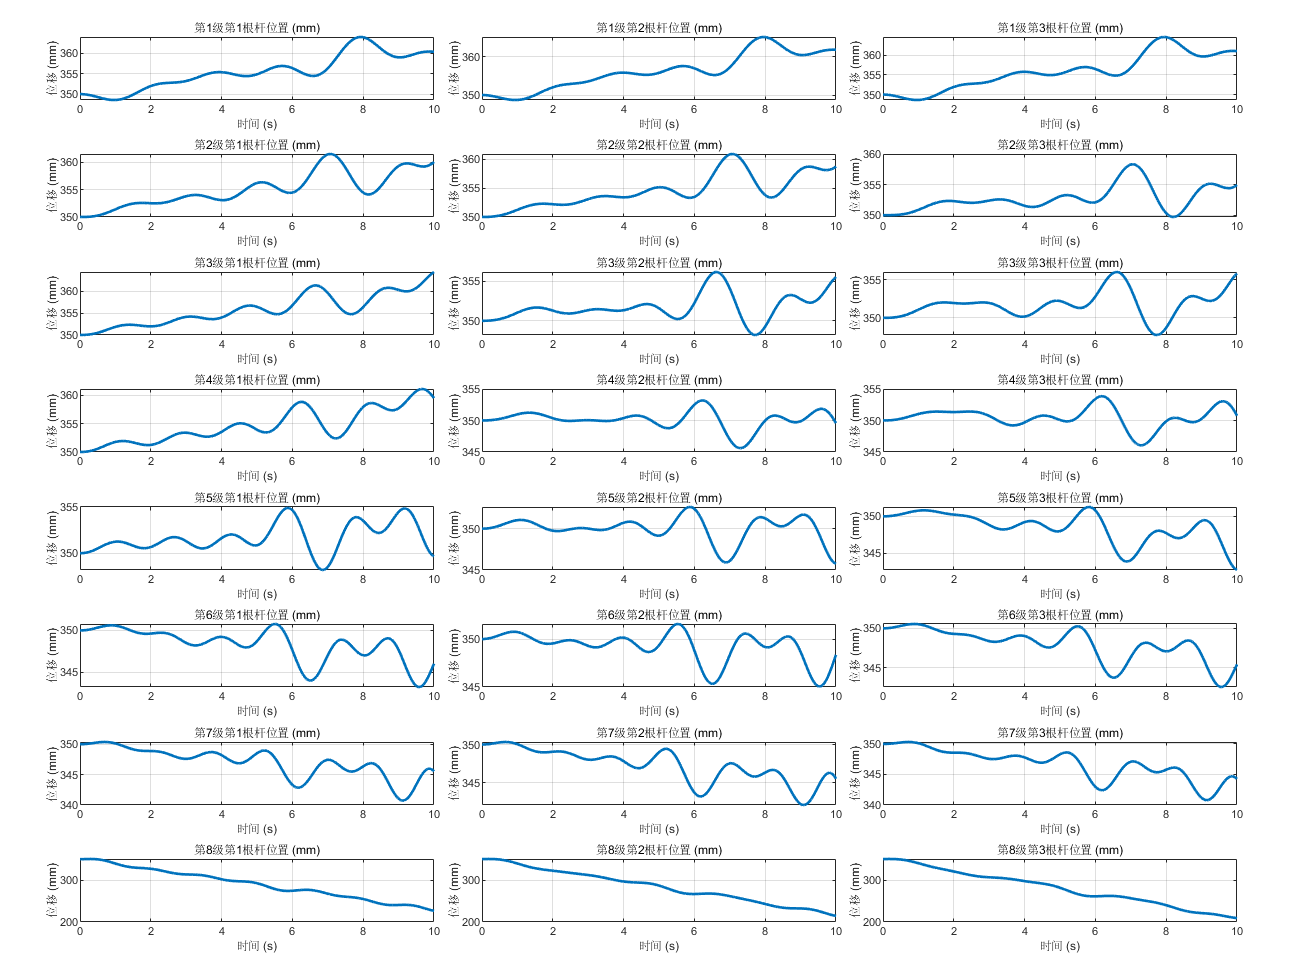
\includegraphics[width=0.95\textwidth]{../结果图示/各级各杆位置变化.png}
    \caption{八级柔性臂各根驱动杆的伸缩响应。横轴为时间，纵轴为杆长增量（毫米）。各级保持初始偏置约 $0.35~\si{\meter}$，在外力激励下呈现渐次衰减的振荡。}
    \label{fig:rod-displacement}
  \end{figure}

  \begin{figure}[H]
    \centering
    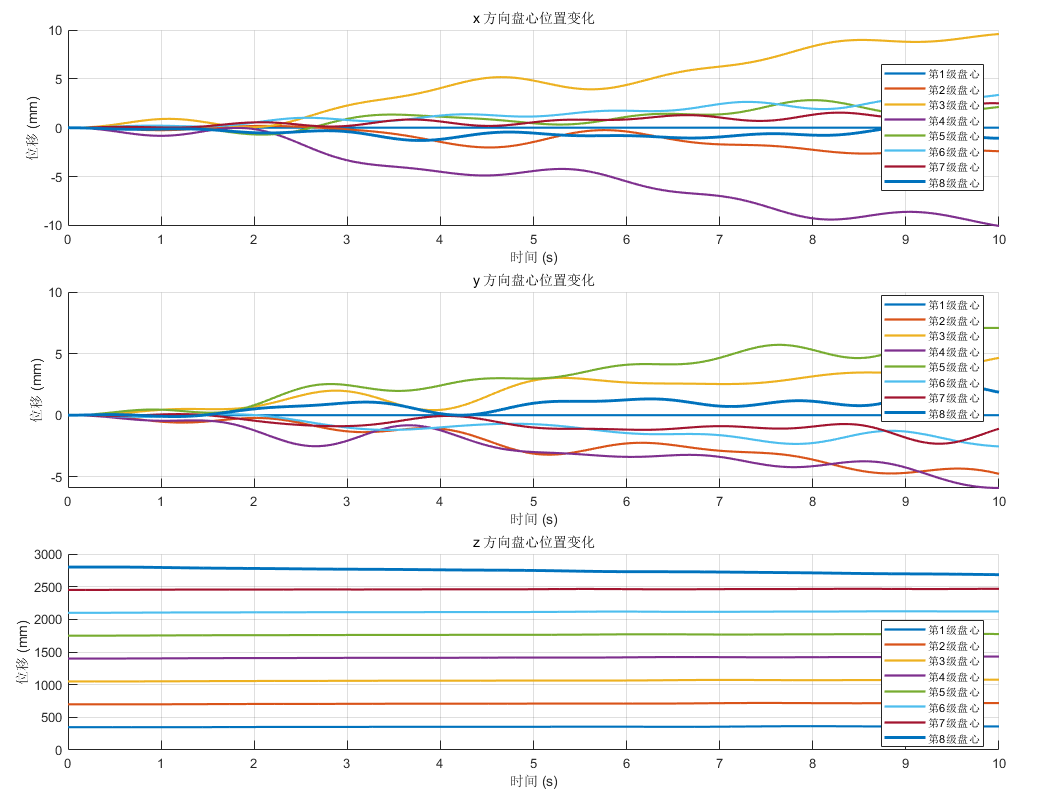
\includegraphics[width=0.95\textwidth]{../结果图示/盘心位置变化.png}
    \caption{各级盘心在 $x$、$y$、$z$ 三个方向上的位移曲线。横轴为时间，纵轴为位移（毫米）。$z$ 方向保持平台高度层级差，$x$ 与 $y$ 方向则体现出外力驱动下的横向漂移与耦合振荡。}
    \label{fig:plate-position}
  \end{figure}

  \begin{figure}[H]
    \centering
    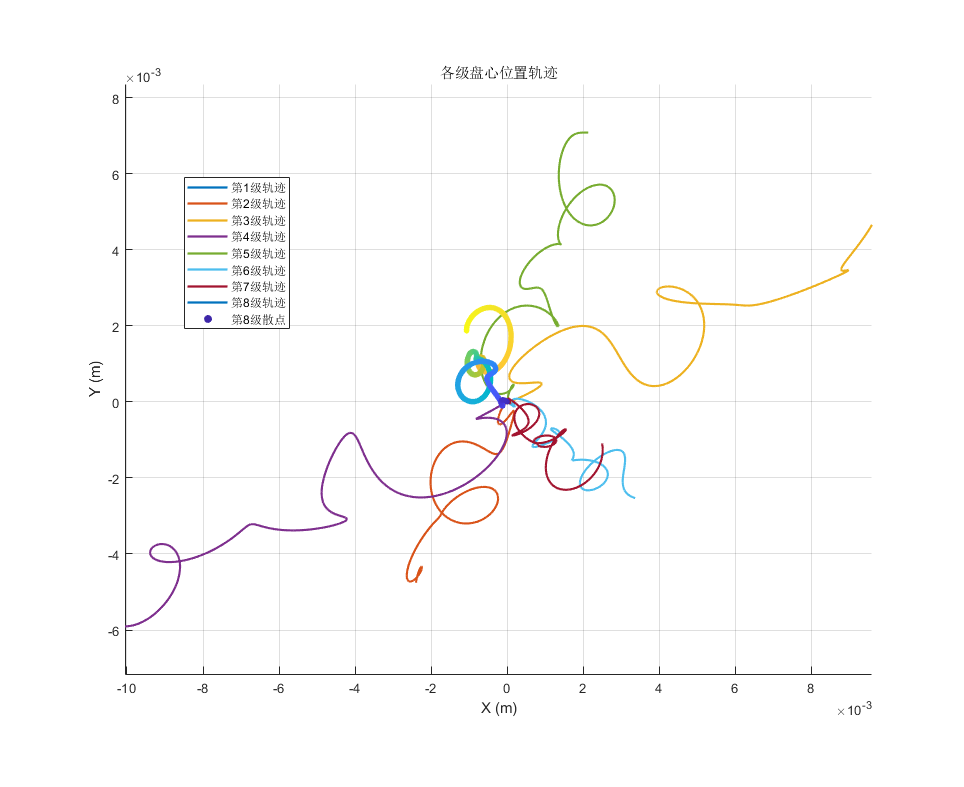
\includegraphics[width=0.72\textwidth]{../结果图示/X-Y平面各级盘心.png}
    \caption{八级盘心在 $x$-$y$ 平面内的空间轨迹。颜色由低级到高级依次区分，可观察到沿级数逐渐展开的螺旋状运动以及末级终端位置。}
    \label{fig:xy-trajectory}
  \end{figure}

\section{结论}
本文档给出了柔性臂单级的齐次变换、角度解算、质量与约束矩阵的构造，并说明了控制力、外力及串联扩展的推导流程，数值实现中加入了矩阵正则化与求解器回退机制以提升稳定性。整体框架可支持多级柔性臂的动力学仿真与控制设计。

\end{document}
